\documentclass[10pt,handout]{beamer}

\usepackage[french]{babel}
\usepackage[T1]{fontenc}
\usepackage[utf8]{inputenc}
\usepackage[
    left = \flqq{},%
    right = \frqq{},%
    leftsub = \flq{},%
    rightsub = \frq{} %
]{dirtytalk} 	% for \say{}
\usepackage{xcolor} 	% for color text
\usepackage{csquotes}
\usepackage{amssymb}
\usepackage{mathtools}
\usepackage{array}

\usetheme{Frankfurt}
\usetheme{CambridgeUS}
\usetheme{JuanLesPins}
%\usetheme{Montpellier}
%\usetheme{Madrid}

\usecolortheme{dolphin}

\useinnertheme{circles}
\usefonttheme{structurebold}
\useoutertheme{default}

%\hypersetup{pdfpagemode=FullScreen}

\title[Chemins spécifiques]{Chemins spécifiques pour la classification dans les réseaux de neurones profonds}
\author[Bouzidi, Elhouiti, Kezzoul, Zeroual, Dadi]{Bouzidi Belkacem - Dadi Mélissa \\ Elhouiti Chakib - Kezzoul Massili \\ Zeroual Ramzi}
\institute[]{Université de Montpellier}
\date{\today}

% Pour inserer une frame de sommaire avant chaque debut de section
\AtBeginSection[]
{
  \placelogofalse
  \begin{frame}
    \tableofcontents[hideothersubsections,currentsection,subsectionstyle=show/shaded/hide]
  \end{frame}
  \placelogotrue
}

% Mettre les listes en triangle
\setbeamertemplate{itemize item}[triangle]

%Insertion d'un logo
\newif\ifplacelogo % create a new conditional
\placelogotrue % set it to true
\logo{\ifplacelogo
\includegraphics[height=12mm]{img/univ-montpellier.png}\fi}

%------------------------------------------------------%
% page de titre
%------------------------------------------------------%
\begin{document}

\placelogofalse
\begin{frame}
	\titlepage
\end{frame}

\placelogotrue

\section{Introduction}
\subsection{Les réseaux de neurones profonds}
\begin{frame}{Les réseaux de neurones profonds}
    
\end{frame}

\placelogofalse 
\subsection{Le jeu de données}
\begin{frame}{MNIST}
    \makebox[\textwidth]{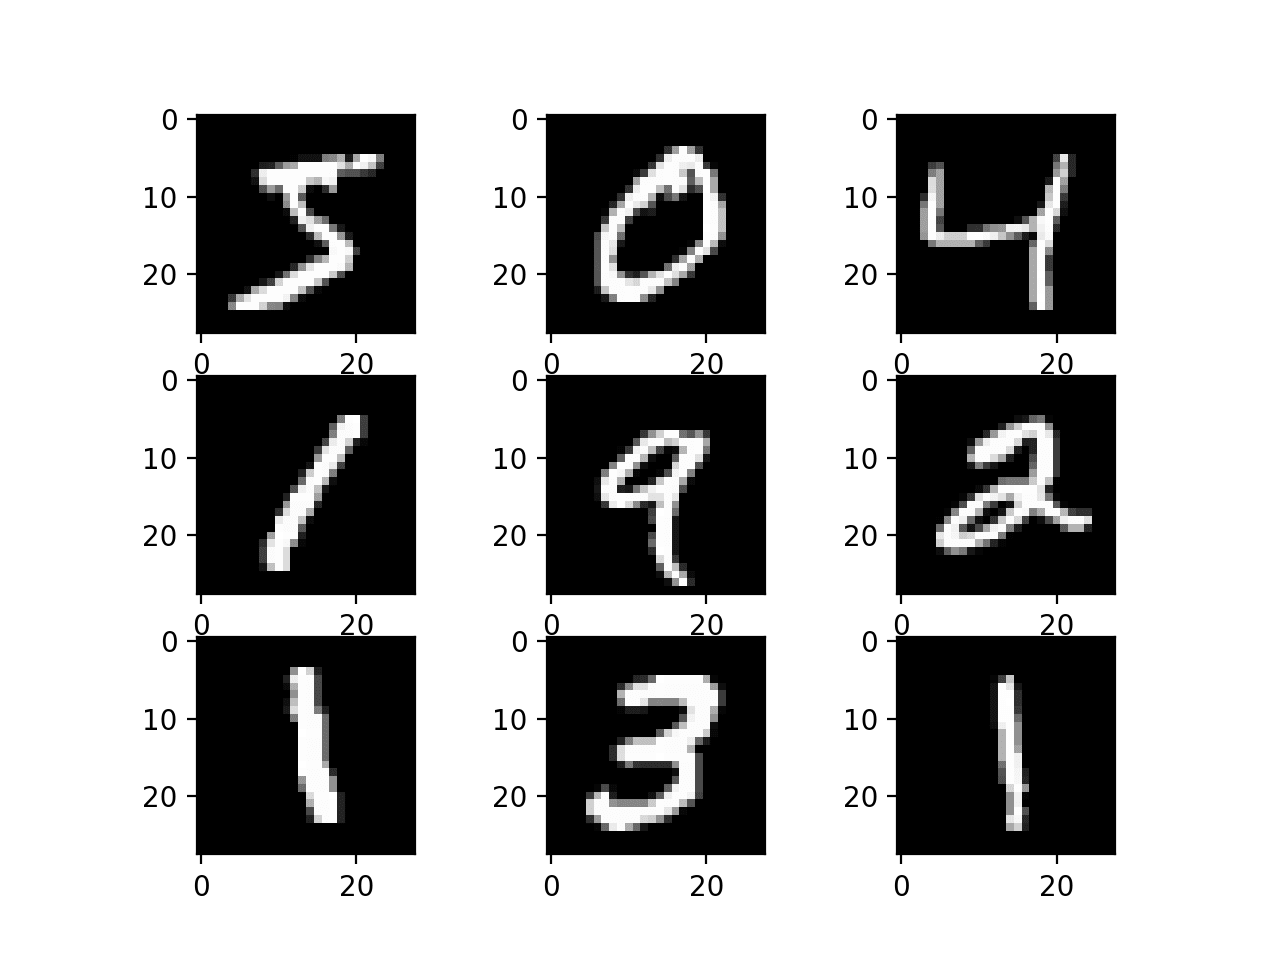
\includegraphics[width=0.8\textwidth]{img/mnist.png}}
\end{frame}
\placelogotrue

\placelogofalse 
\subsection{Problèmatique}
\begin{frame}{Problèmatique}
    \begin{block}{Boite noire}
        Les réseaux de neurones semblent s'appliquer à la manière d'une boite noire. Aucune information n'est fournie sur ce qui les a conduits à atteindre leurs prédictions.
    \end{block}
    \begin{block}{Objectifs}
        L'objectif est de comprendre le fonctionnement interne d'un réseau de neurones et de repérer des signatures d'activation de neurones en variant les données.
    \end{block}

    \makebox[\textwidth]{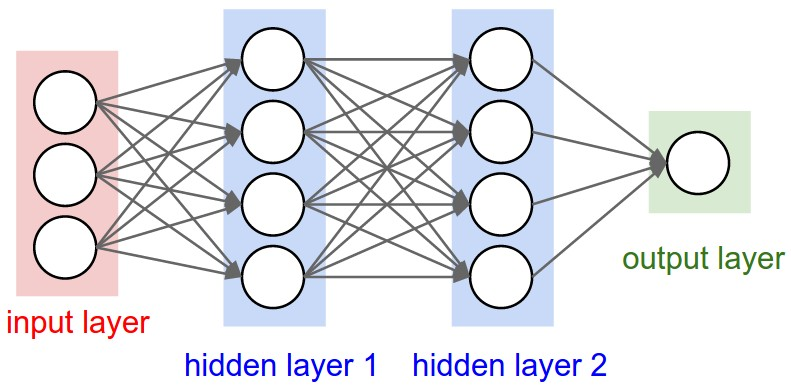
\includegraphics[width=0.6\textwidth]{img/ann-dense.jpg}}
        
\end{frame}
\placelogotrue

\begin{frame}{Questions qu'on se posent}
    Par exemple, si on entraîne un modèle à reconnaître des images de 1 et de 7
    \begin{itemize}
        \item À partir de quelle couche le modèle change de comportement pour reconnaître une image ?
        \item Les signatures des images de \textit{7}, sont-elles différentes de ceux des \textit{1} ?
        \item Si on passe une image de \textit{3} au modèle, à quoi va ressembler sa signature ?
    \end{itemize}    
\end{frame}

\subsection{Solution proposée}
\begin{frame}{Solution proposée}
    \begin{itemize}
        \item Construire des réseaux de neurones.
        \item Récupérer, pour chaque donnée, la sortie des couches cachées.
        \item Extraire les signatures grâce à des algorithmes de \textit{clustering}.
        \item Réaliser une interface de visualisation en utilisant différentes techniques.
        \item Analyser les résultats et répondre aux questions.
    \end{itemize}
\end{frame}

\section{Organisation}
\begin{frame}{Organisation du projet}
    
\end{frame}

\section{Analyse des données}
\begin{frame}
    \begin{block}{Importance de l'analyse}
        L'objectif de l'analyse des données, c'est de savoir comment sont nos données et comment on peut les utiliser.
    \end{block}
\end{frame}
 

\subsection{Découpage des données}

\begin{frame}{Découpage des données}
    \begin{itemize}
        \item Garder un nombre précis d’images pour un ensemble de chiffres définis.
        \item Faciliter la phase de développement.
        \item Pouvoir mieux visualiser les résultats sur un petit
        ensemble de données.
    \end{itemize}
\end{frame}

\subsection{Prétraitement}
\begin{block}{Scaling}
    Utilisation de la normalisation, qui consiste à
    mettre les valeurs des images entre 0 et 1 au lieu de 0 et 255.
\end{block}
\begin{block}{Flattening}
    Aplatissement des images pour avoir un tableau à une seule dimension au lieu d’une matrice à deux dimensions.
\end{block}
\begin{block}{}
    Transformation des labels en un vecteur binaire contenant que des 0 et des 1.
    \begin{itemize}
        \item Taille du vecteur égale au nombre de labels uniques à garder.
        \item Tri des labels à garder.
        \item Mettre un 1 à la case du label correspendant
        et des 0 aux autres cases.
        \item Ex: transformation en vecteur des images de 1, 3 et 7.
        \item Pour un 1 $\implies$ [1,0,0].
        \item Pour un 3 $\implies$ [0,1,0].
        \item Pour un 7 $\implies$ [0,0,1].
    \end{itemize}
\end{block}

\section{Développement de l’architecture}
\subsection{Technologies utilisées}
\begin{frame}{Jupyter notebook}
    
\end{frame}

\begin{frame}{Tensorflow, Keras}
    
\end{frame}

\begin{frame}{Voilà}
    \begin{block}{}
        Voilà permet de transformer un
        notebook jupyter en une application web autonome (standalone).
    \end{block}
    \begin{block}{}
        Voilà permet aussi de changer l’interface graphique de la page d’accueil grâce à des templates.
    \end{block}    
\end{frame} 

\placelogofalse 
\subsection{Modèle d'apprentissage}
\begin{frame}{Modèle d'apprentissage}
    \begin{block}{Types de réseau}
        Les types de réseau diffèrent par plusieurs paramètres :
        \begin{itemize}
            \item la topologie des connexions entre les neurones ;
            \item la fonction d’agrégation utilisée;
            \item et bien d’autres paramètres.
        \end{itemize}
    \end{block}

    \makebox[\textwidth]{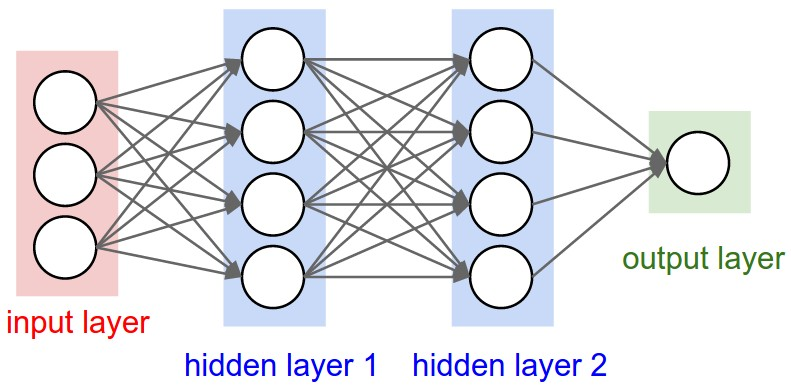
\includegraphics[width=0.6\textwidth]{img/ann-dense.jpg}}
\end{frame}
\placelogotrue 

\begin{frame}{Réseau de neurones à convolution}
    \makebox[\textwidth]{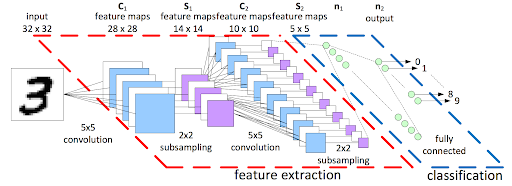
\includegraphics[width=0.9\textwidth]{img/cnn.png}}
\end{frame}

\placelogofalse 
\subsection{Signature et Clustering}
\begin{frame}{Signature}
    \begin{block}{Définition}
        Soit un réseau à $N$ couches cachées, La \textit{signature} $S$ d'une image qui travesent ce réseau, se définit ainsi : $ S = (H_1, ..., H_N) $, avec $H_i$ est le vecteur contenant les valeurs de chaque neurone de la couche $i$.
    \end{block}
    \makebox[\textwidth]{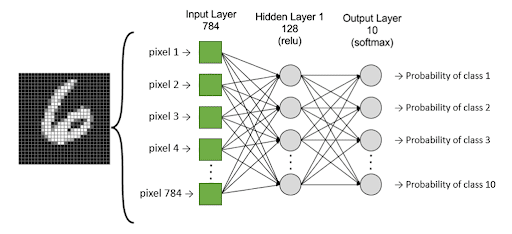
\includegraphics[width=0.8\textwidth]{img/dense-mnist.png}}
\end{frame}
\placelogotrue 

\placelogofalse 
\begin{frame}{Clustering}
    \begin{block}{K-means}
        \textbf{K-means} est algorithme de \textit{clustering}. Il prend en paramètres les
        données et un certain $K$ donnée par l’utilisateur, puis construit $K$ clusters qui regroupent les données qui sont proches (en terme de distance euclidienne).
    \end{block}
    \makebox[\textwidth]{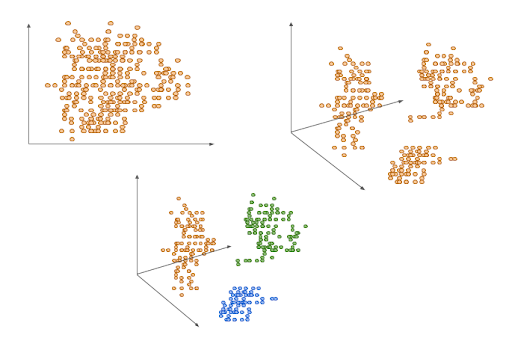
\includegraphics[width=0.6\textwidth]{img/kmeans.png}}
\end{frame}
\placelogotrue 

\begin{frame}{Score \textit{Silhouette}}
    \begin{block}{Choisir un $K$}
        Par contre, l'algorithme ne permet pas de trouver tout seul un $K$ optimal. Mais il existe une méthode qui calcul la performance d'un \textit{clustering}. La méthode \textit{Silhouette}.
    \end{block}
    \begin{block}{Score \textit{Silhouette}}
        Concrétement, cette méthode consiste à calculer pour un clustering, la moyenne du score \textit{Silhouette} de chaque point. $ s(i) = \frac{b(i) - a(i)}{max(a(i), b(i))} $.

        Avec $a(i)$ est la mesure de la similarité du point $i$ avec son cluster et $b(i)$ le mesure de dissemblance du point $i$ par rapport aux autres clusters.
    \end{block}
\end{frame}

\begin{frame}
    \makebox[\textwidth]{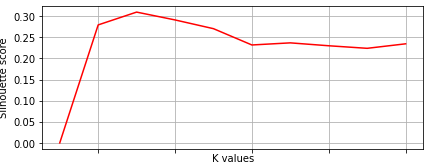
\includegraphics[width=0.9\textwidth]{img/silhouette.png}}
\end{frame}

\subsection{Interface de visualisation}
\placelogofalse
\begin{frame}{UMAP }
    \begin{block}{UMAP}
        (Uniform Manifold Approximation and Projection) Utilise des algorithmes de mise en page graphique pour organiser les données dans
        un espace de faible dimension.
    \end{block}
    \makebox[\textwidth]{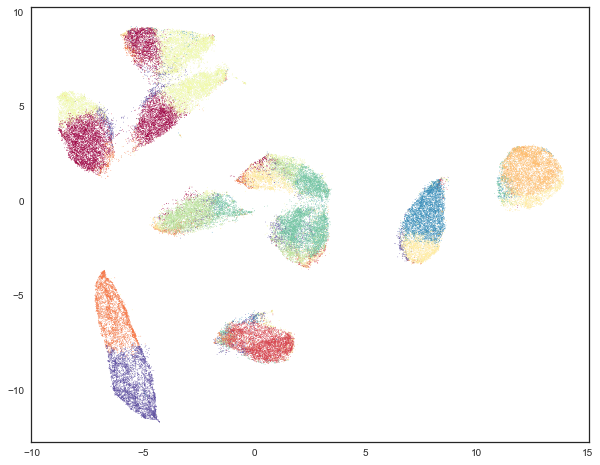
\includegraphics[width=0.6\textwidth]{img/UMAP.png}}

\end{frame}
\placelogotrue

\begin{frame}{Diagramme de Sankey}
    \begin{block}{}
        Un diagramme de Sankey est un type de diagramme de flux 6 dans lequel la largeur des flèches
        est proportionnelle au flux représenté.
    \end{block}
    \makebox[\textwidth]{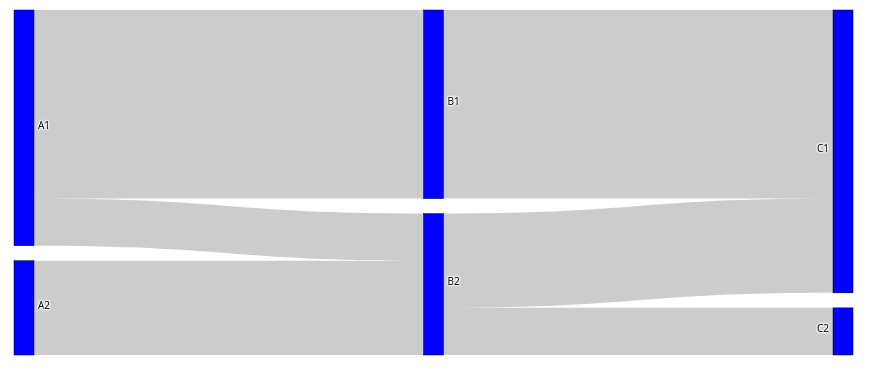
\includegraphics[width=0.6\textwidth]{img/sankey.png}}
\end{frame}
\placelogofalse
\begin{frame}{Application web}
    \begin{block}{Page web}
        Transformation d'un Jupyter notebook contenant les différentes visualisations et faisant le lien entre eux.
    \end{block}
    \makebox[\textwidth]{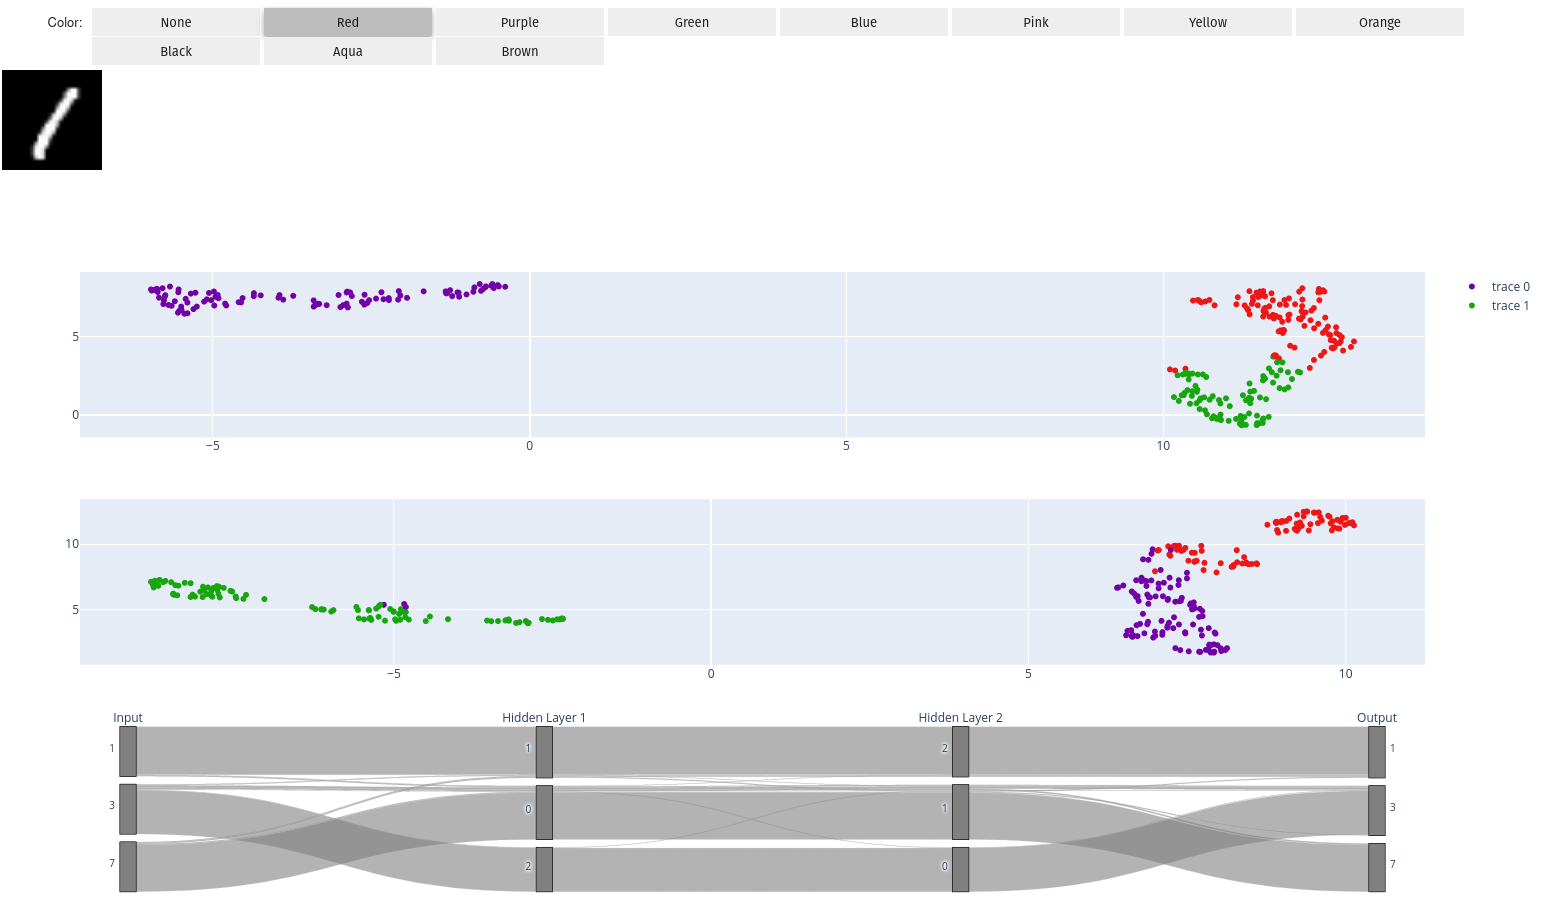
\includegraphics[width=0.8\textwidth]{img/umap-sankey2.png}}
\end{frame}

\begin{frame}{Application web}
    \begin{block}{Page d'accueil}
        Création d'une page d'accueil personnalisée présentant nos différentes expérimentations.
    \end{block}
    \makebox[\textwidth]{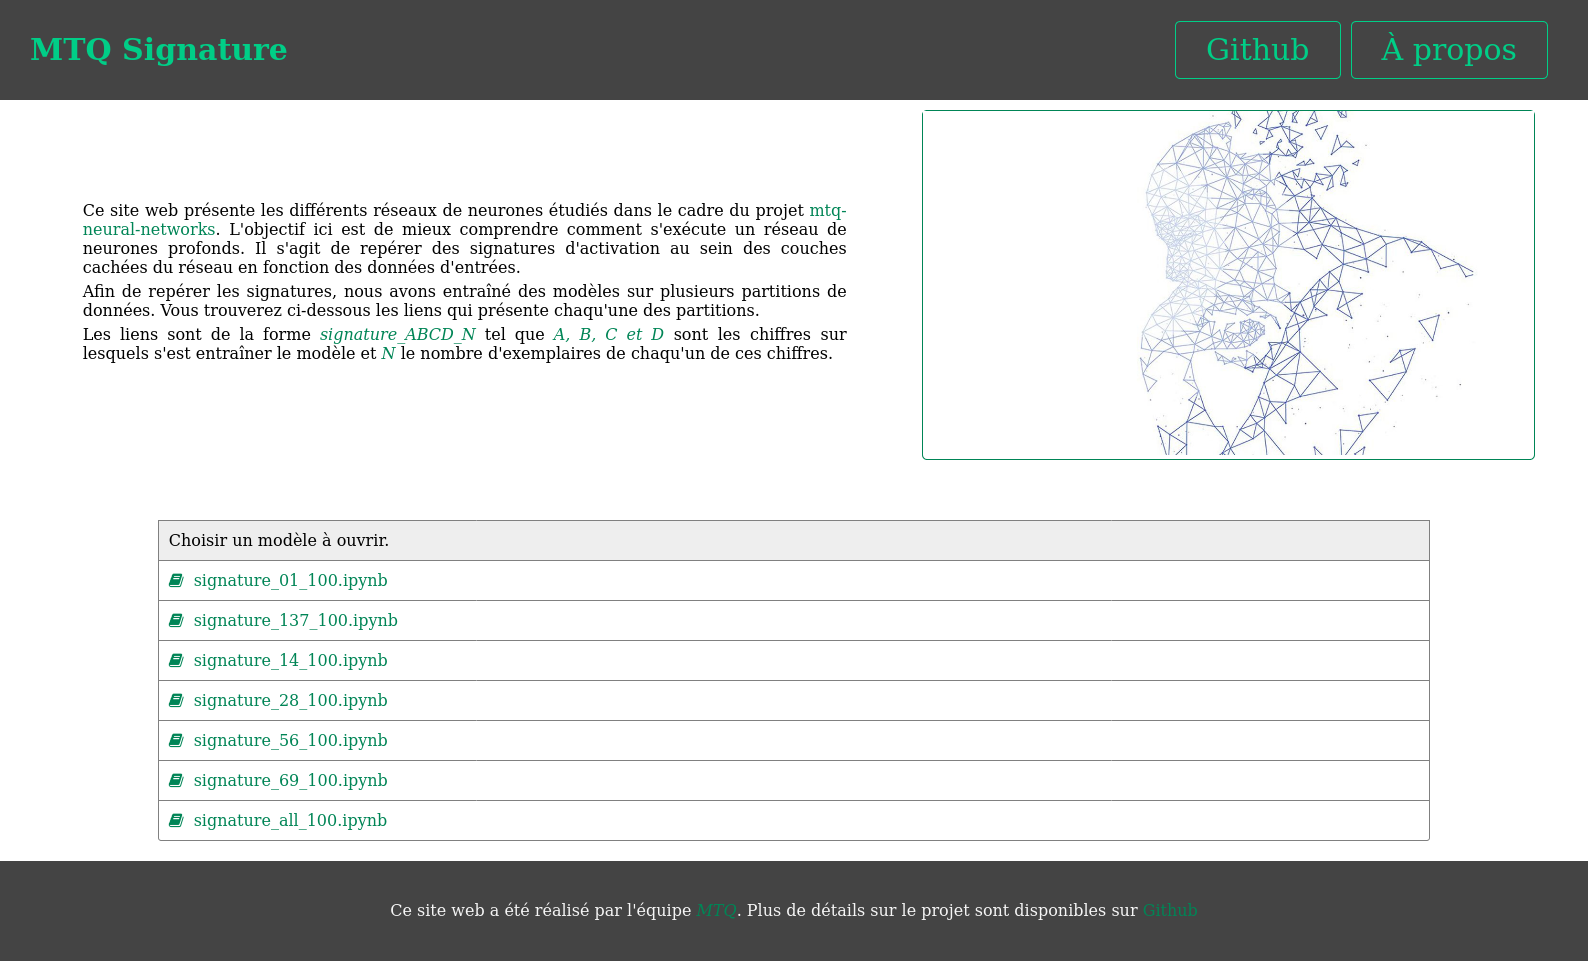
\includegraphics[width=0.8\textwidth]{img/accueil.png}}
\end{frame}
\placelogotrue



\section{Analyse des résultats}
\begin{frame}{Résultat}
    \begin{block}{}
        Afin d'illuster les résultats obtenu, nous prenons un exemple oû on entraine un modèle à deux couches cachées à reconnaitre des images de \textit{1} et de \textit{7}.
    \end{block}
\end{frame}

\placelogofalse
\begin{frame}{Résultats}
    \makebox[\textwidth]{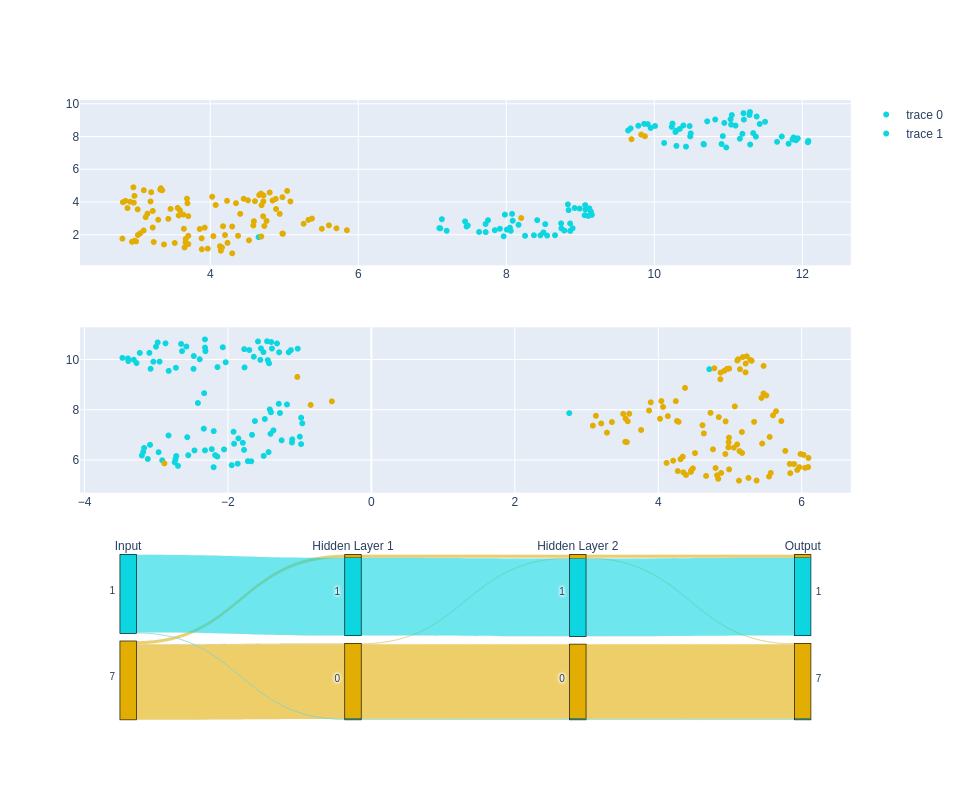
\includegraphics[width=0.8\textwidth]{img/visualisation17.png}}
\end{frame}
\placelogotrue

\subsection{Réponses aux questions}
\begin{frame}{Changement de comportement}
    %À partir de quelle couche le modèle change de comportement pour reconnaître une image ?
    \begin{block}{}
        Notre modèle arrive, dès la première couche cachée, à reconnaître une image.
    \end{block}
    
    \makebox[\textwidth]{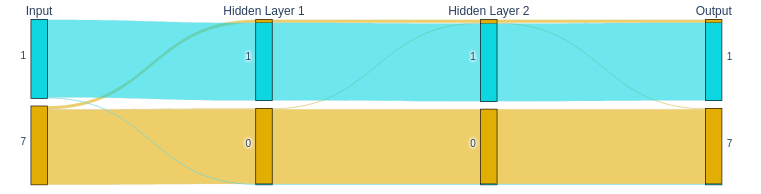
\includegraphics[width=0.8\textwidth]{img/sankey17.png}}
\end{frame}

\begin{frame}{Différence de signatures}
    %Les signatures des images de 7, sont-elles différentes de ceux des 1 ?
    \begin{block}{}
        On observe que les signatures des 1 sont majoritairement différentes de celles des 7. Sauf pour quelques rares exceptions.
    \end{block}

    \makebox[\textwidth]{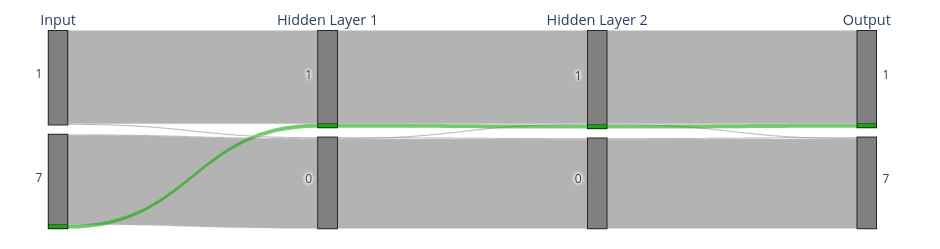
\includegraphics[width=0.8\textwidth]{img/sankey_7.png}}

\end{frame}

\begin{frame}
    \begin{figure}[h]
        \begin{minipage}[c]{.46\linewidth}
        \centering
        
\includegraphics[width=0.4\textwidth]{img/7_1.png}
        \end{minipage}
        \hfill%
        \begin{minipage}[c]{.46\linewidth}
        \centering
        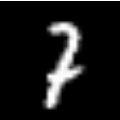
\includegraphics[width=0.4\textwidth]{img/7_2.png}
        \end{minipage}
        \end{figure}
        
        \begin{figure}[h]
        \begin{minipage}[c]{.46\linewidth}
        \centering
        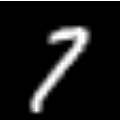
\includegraphics[width=0.4\textwidth]{img/7_3.png}
        \end{minipage}
        \hfill%
        \begin{minipage}[c]{.46\linewidth}
        \centering
        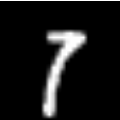
\includegraphics[width=0.4\textwidth]{img/7_4.png}
        \end{minipage}
        \caption{Les images de 7 ressemblant à des 1}
        \label{71}
    \end{figure}
\end{frame}

\begin{frame}{Insertion d’anomalies}
    %Si on passe une image de 3 au modèle, à quoi va ressembler sa signature ?
    \begin{figure}[h]
        \centering
        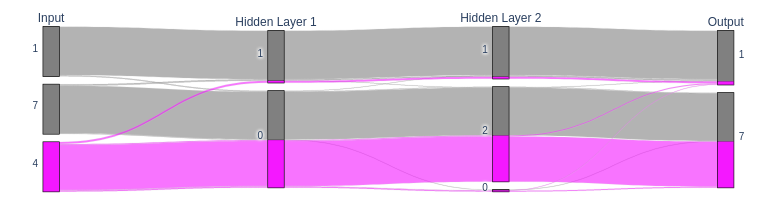
\includegraphics[width=0.9\textwidth]{img/anomalie4_sankey.png}
        \caption{Insertion d’images de 4}
    \end{figure}
\end{frame}

\begin{frame}{Insertion d’anomalies}
    %Si on passe une image de 3 au modèle, à quoi va ressembler sa signature ?
    \begin{figure}[h]
        \centering
        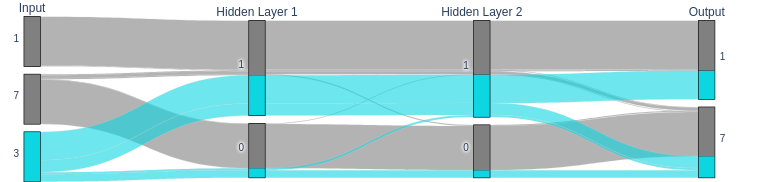
\includegraphics[width=0.9\textwidth]{img/anomalie3_sankey.png}
        \caption{Insertion d’images de 3}
    \end{figure}
\end{frame}

\subsection{Conclusion}
\begin{frame}{Conclusion}
    \begin{block}{}
        Soit $n$ attributs de $A_1$ à $A_n$. On cherche à entraîner un modèle à classifier ces données en deux classes $C_1$ et $C_2$. Le modèle peut détecter des similarités entre les objets sur un attribut $A_i$ qui indique qu'il existe peut-être \textit{une corrélation}, mais pas forcément \textit{une causalité}, avec les deux classes $C_1$ et $C_2$. Ce qui mènera notre modèle à de possibles mauvaises classifications sur des données qu'il n'a jamais vues.
    \end{block}
\end{frame}


\begin{frame}
    \begin{center}
      Merci pour votre attention.
    \end{center}
\end{frame}
  
\end{document}